\chapter{Resultados}

\section{Resultados de Simulação Computacional}

\subsection{Inversor como STATCOM}

O primeiro teste realizado foi o de verificar a operação do inversor trifásico conectado 
à rede elétrica sem injeção de potência no barramento CC. A referência de tensão estabelecida foi de 680 V.
A Fig. \ref{fig:sim-circuito-statcom} mostra o circuito utilizado.

\begin{figure}[!hbt]
	\begin{center}
    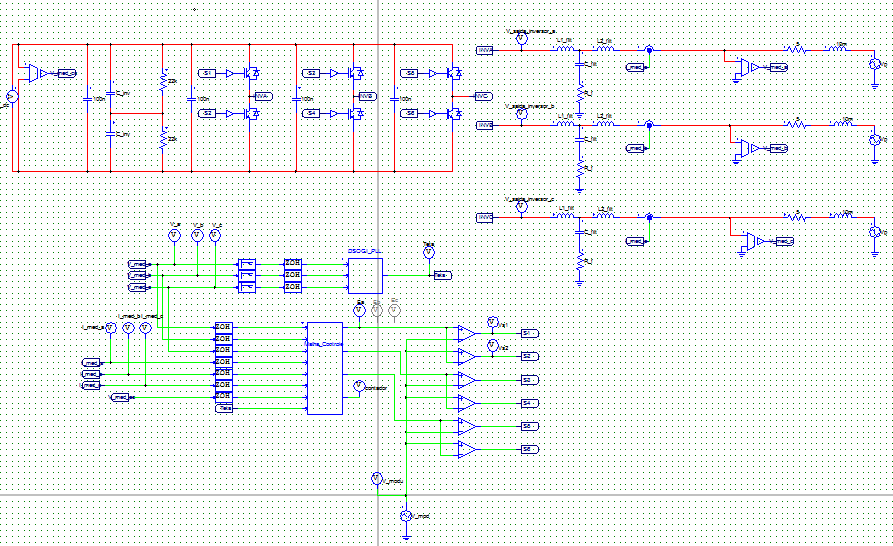
\includegraphics[width=\textwidth]{figuras/sim_figures/statcom/circuito.PNG}
    \caption{Circuito do inversor conectado à rede elétrica na operação como STATCOM no \textit{software} PSIM}
    \label{fig:sim-circuito-statcom}
    \end{center}
\end{figure}

Ao se iniciar a simulação, o barramento CC do inversor é carregado por 100 ms sem a atuação do controle. 
Após isto, o sinais de PWM são enviados para a realização do chaveamento, e as tensões e correntes são enviadas para o circuito de controle do inversor.
Na Fig. \ref{fig:sim-statcom} pode-se verificar os resultados para o barramento CC e a sintetização de tensões da rede.
A tensão no barramento fica estabilizada em aproximadamente 3 segundos e a sintetização correta das tensões e correntes é realizada.

\begin{figure}[!hbt]
	\centering
	\begin{subfigure}[b]{0.49\textwidth}
		\centering
		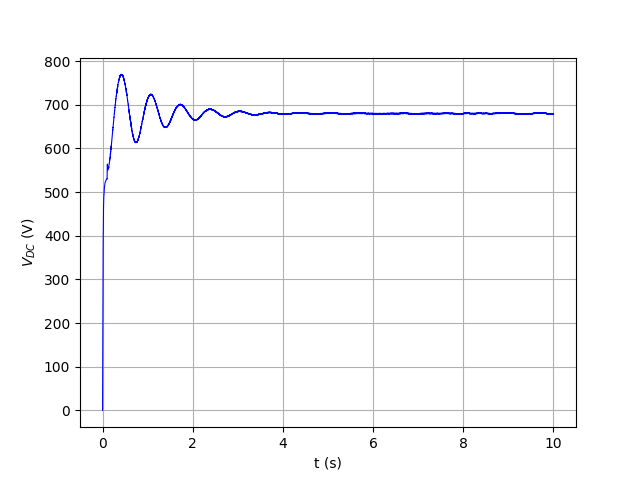
\includegraphics[width=\textwidth]{figuras/sim_figures/statcom/barramento-cc.png}
		\caption{ }
	\end{subfigure}
	\begin{subfigure}[b]{0.49\textwidth}
		\centering
		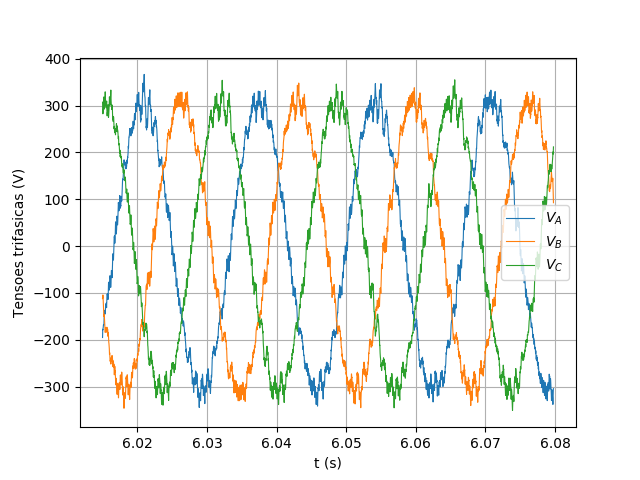
\includegraphics[width=\textwidth]{figuras/sim_figures/statcom/tensoes_trifasicas.png}
		\caption{ }
	\end{subfigure}

	\caption{Resultados de simulação para a operação como STATCOM: (a) Tensão no barramento de corrente contínua. (b) Tensões trifásicas sintetizadas.}
    \label{fig:sim-statcom}
\end{figure}

A Fig. \ref{fig:sim-statcom2} apresenta o ângulo $\theta$, que é o ângulo de fase resultante obtido pelo algoritmo da PLL para obtenção da fase da rede elétrica, 
em comparação com a tensão da rede $V_A$, mostrando que estes estão perfeitamente em fase e que o algoritmo de controle está em sincronia com as tensões da rede.
Além disso, mostra também o resultado do chaveamento a ser enviado para o IGBT e a modulante $e_a$ para um certo trecho de simulação.

\begin{figure}[!hbt]
	\centering
	\begin{subfigure}[b]{0.49\textwidth}
		\centering
		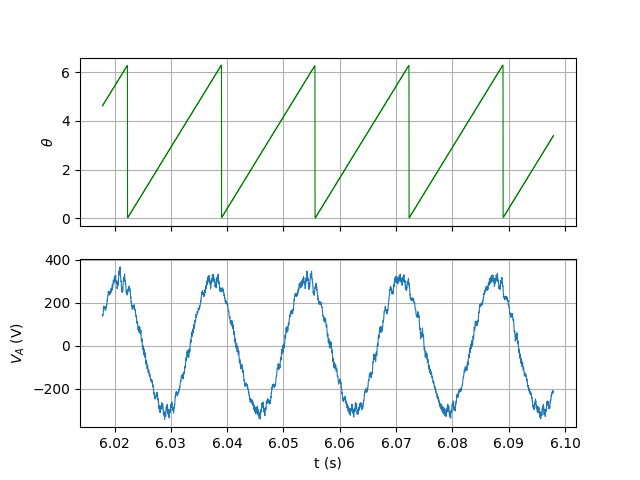
\includegraphics[width=\textwidth]{figuras/sim_figures/statcom/teta.png}
		\caption{}
	\end{subfigure}
	\begin{subfigure}[b]{0.49\textwidth}
		\centering
		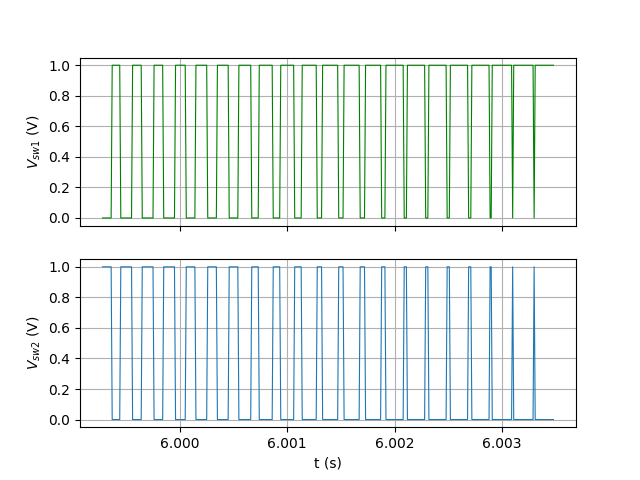
\includegraphics[width=\textwidth]{figuras/sim_figures/statcom/pwm.png}
		\caption{}
	\end{subfigure}
	\begin{subfigure}[b]{0.49\textwidth}
		\centering
		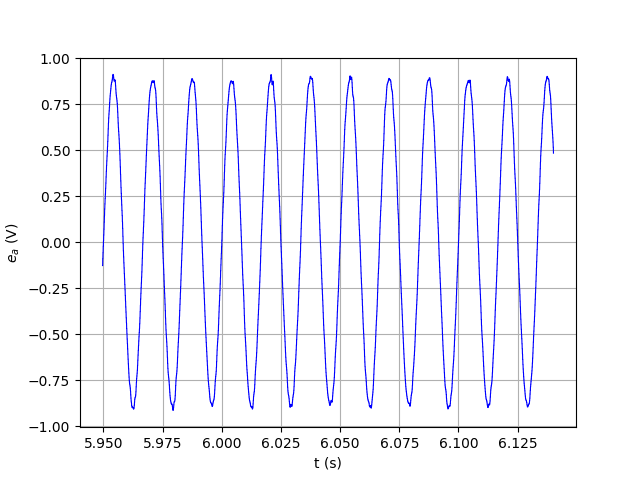
\includegraphics[width=\textwidth]{figuras/sim_figures/statcom/modulante.png}
		\caption{}
	\end{subfigure}

	\caption{Resultados de funcionamento do sistema para a operação como STATCOM: (a) Comparação do ângulo sintetizado pelo algoritmo da PLL e a tensão de fase $V_A$. (b) Sinais de PWM enviados para o braço A do inversor trifásico. (c) Sinal da modulante $e_a$ implementado para ser enviado ao circuito de geração do PWM}
    \label{fig:sim-statcom2}
\end{figure}

A configuração como STATCOM é útil para que a tensão no barramento CC fique estabilizada antes da injeção de potência no barramento, 
e será explorada nas outras etapas de simulação como o passo inicial antes da injeção de potência no sistema.

\subsection{Inversor conectado ao conversor \textit{boost}}

Nesta etapa de simulação, o objetivo foi verificar se o inversor trifásico, juntamente com sua malha de controle, conseguiam realizar transmissão de potência ativa do barramento CC para a rede elétrica. 
Para isto, conectou-se o do barramento de CC à um conversor do tipo \textit{boost}, que injetava corrente no barramento.
O inversor, de forma a manter a tensão no barramento CC constante, realizava as iterações em seu algorítmo de controle de forma a injetar na rede elétrica a corrente recebida.
A Fig. \ref{fig:sim-circuito-inversor-boost} mostra o circuito utilizado.

\begin{figure}[!hbt]
	\begin{center}
    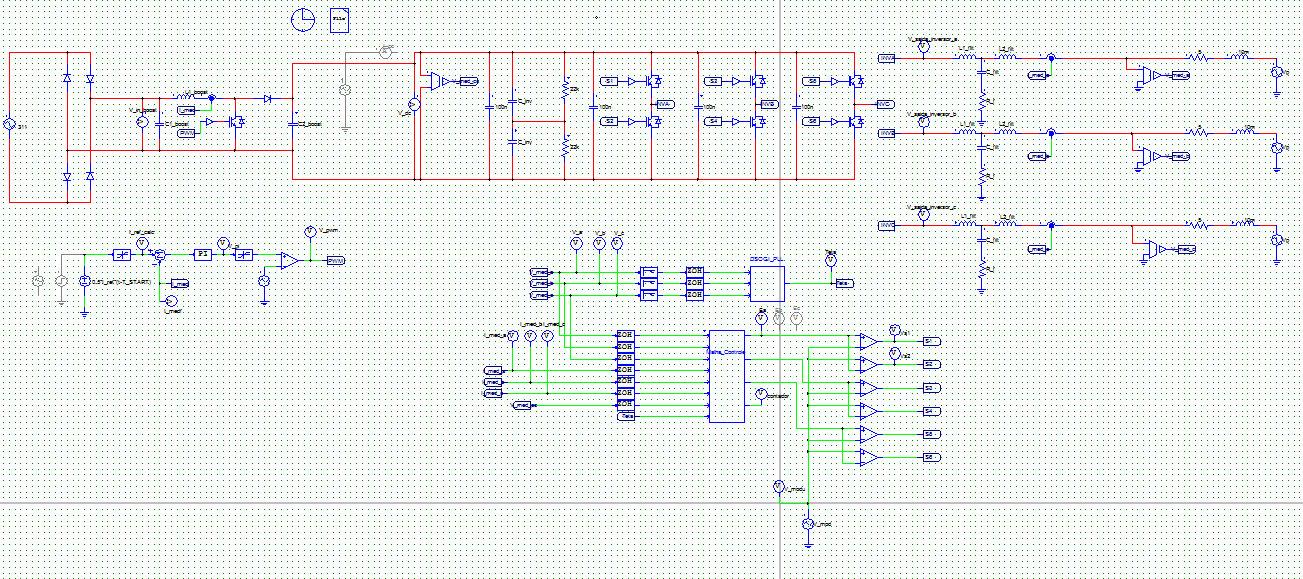
\includegraphics[width=\textwidth]{figuras/sim_figures/inversor_e_boost/esquematico.PNG}\centering
    \caption{Circuito do inversor conectado com o conversor \textit{boost}, juntamente com os blocos de controle no software PSIM}
    \label{fig:sim-circuito-inversor-boost}
    \end{center}
\end{figure}

A tensão de referência definida para o barramento CC foi de 680 V. Desta forma, esperou-se que, apesar das pertubações a serem inseridas no sistema, este conseguisse estabilizar a tensão do barramento CC pŕoximo a tensão de referência após alguns segundos.
Inicialmente o sistema foi inicializado sem nenhuma injeção de potência no barramento CC e permaneceu assim até 1,5 segundos. Após, isso iniciou-se a injeção de potência através do conversor \textit{boost}, que foi programado para injetar 10 A de corrente.

Pode-se verificar na Fig. \ref{fig:sim-tensao-barramento} a estabilização de tensão no barramento CC. 
Antes dos 1,5 segundos, o sistema passou por um transitório, mas conseguiu manter a tensão no barramento próximo de 680 V. 
Após isto, houve a inserção de corrente pelo \textit{boost}, que provocou uma pertubação, de forma a elevar a tensão sobre o \textit{link} capacitivo do barramento.
De forma a estabilizar esta tensão, o sistema começou a fornecer potência à rede elétrica de modo a manter a tensão CC próximo a seu valor de referência.

\begin{figure}[!hbt]
	\begin{center}
    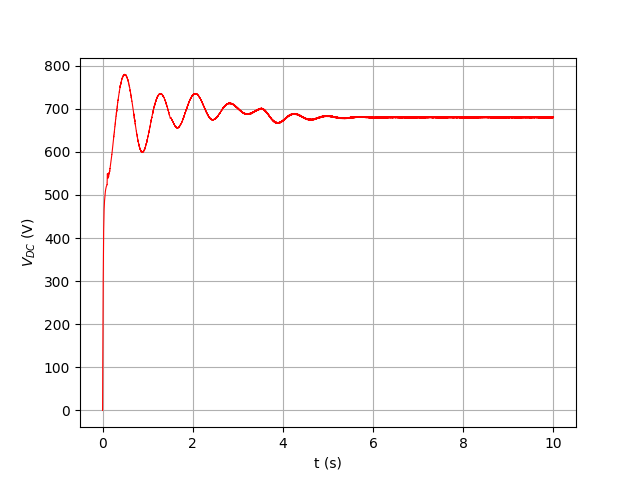
\includegraphics[width=0.5\textwidth]{figuras/sim_figures/inversor_e_boost/tensao_barramento.png}
    \caption{Tensão no barramento CC com a conexão do inversor com o conversor \textit{boost}.}
    \label{fig:sim-tensao-barramento}
    \end{center}
\end{figure}

A Fig. \ref{fig:sim-tensao-saida-inversor} mostra as tensões sintetizadas na saída do inversor, após o filtro $L_2$.
Ao se verificar o espectro em frequência da tensão sintetizada na fase $V_A$, é possível ver que existem harmônicas 
perto da frequência de chaveamento, mas que não produzem alterações significativas na tensão de saída. 
Verifica-se ainda que houve a sintetização correta das tensões em cada fase.

\begin{figure}[!hbt]
	\centering
	\begin{subfigure}[b]{0.49\textwidth}
	\centering
		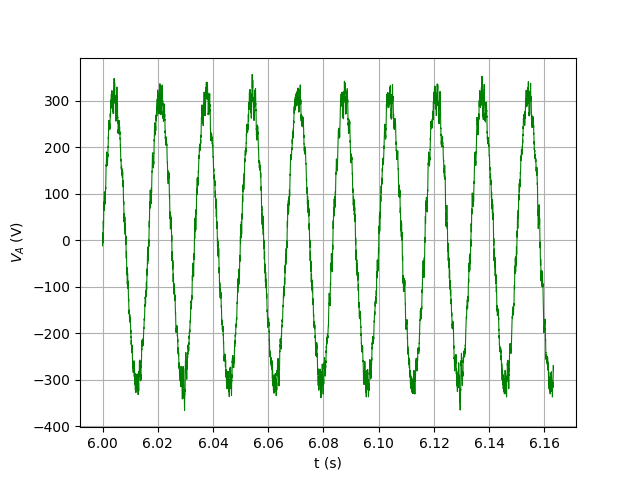
\includegraphics[width=\textwidth]{figuras/sim_figures/inversor_e_boost/tensao_va.png}
		\caption{}
   \end{subfigure}
   \begin{subfigure}[b]{0.49\textwidth}
	\centering
		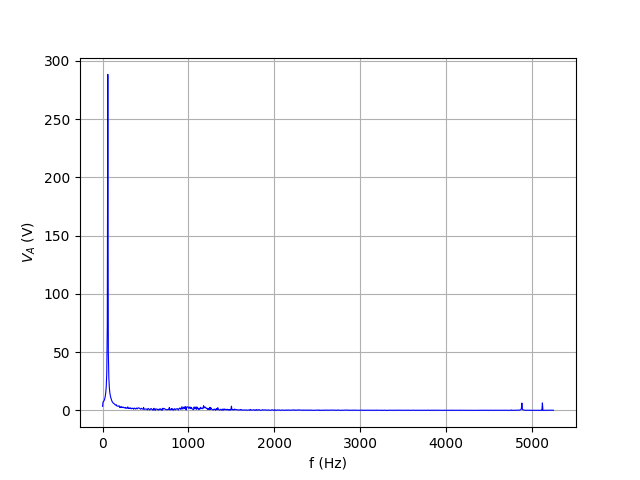
\includegraphics[width=\textwidth]{figuras/sim_figures/inversor_e_boost/tensao_va_espectro.png}
		\caption{}
   \end{subfigure}
	\begin{subfigure}[b]{0.49\textwidth}
	\centering
		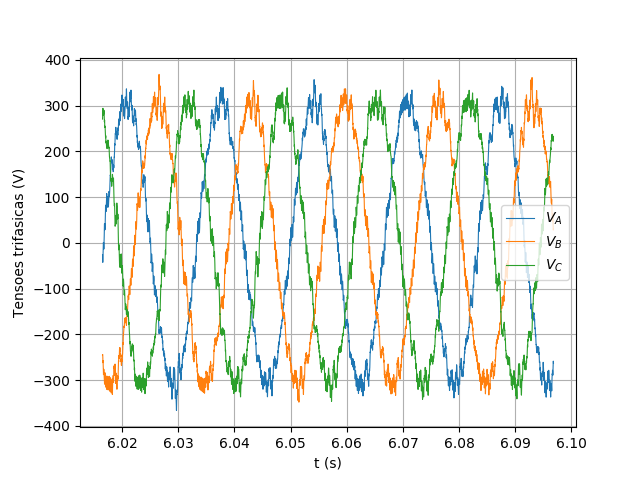
\includegraphics[width=\textwidth]{figuras/sim_figures/inversor_e_boost/tensao_va_vb_vc.png}
		\caption{}
	\end{subfigure}
    \caption{Análise das tensões de saída sintetizadas após o filtro LCL: (a) Tensão de saída sintetizada para a fase A. (b) Espectro em frequência da tensão sintetizada na fase A. (c) Tensões de saída sintetizadas para as fases A, B e C.}
    \label{fig:sim-tensao-saida-inversor}
\end{figure}

Já a Fig. \ref{fig:sim-corrente-saida-inversor} mostra as correntes geradas após a inserção de potência 
pelo \textit{boost} no barramento CC.
O espectro em frequência da corrente produzida na fase A denominada $I_A$ mostra que existem 
harmônicas de baixa frequência, de quinta e sétima ordem, mas que não provocam alterações 
significativas na corrente produzida. Ainda é possível verificar o envio correto das três 
correntes para a rede elétrica.

\begin{figure}[ht]
\centering
 	\begin{subfigure}[b]{0.49\textwidth}
 		\centering
 		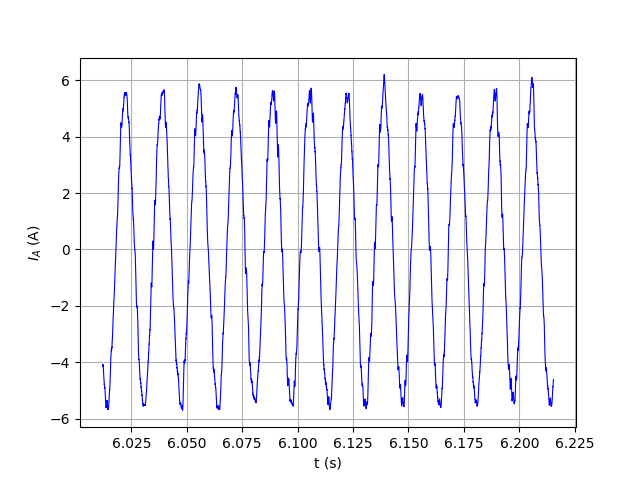
\includegraphics[width=\textwidth]{figuras/sim_figures/inversor_e_boost/corrente_ia.png}
 		\caption{}
	\end{subfigure}
     \begin{subfigure}[b]{0.49\textwidth}
  		\centering
  		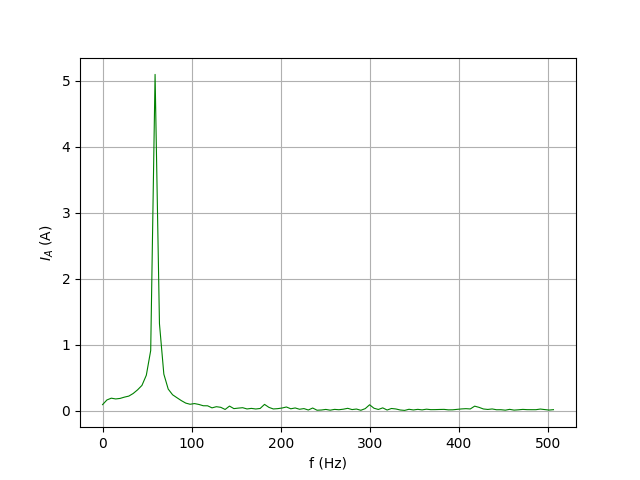
\includegraphics[width=\textwidth]{figuras/sim_figures/inversor_e_boost/corrente_ia_espectro.png}
  		\caption{}
 	\end{subfigure}
  	\begin{subfigure}[b]{0.49\textwidth}
  		\centering
  		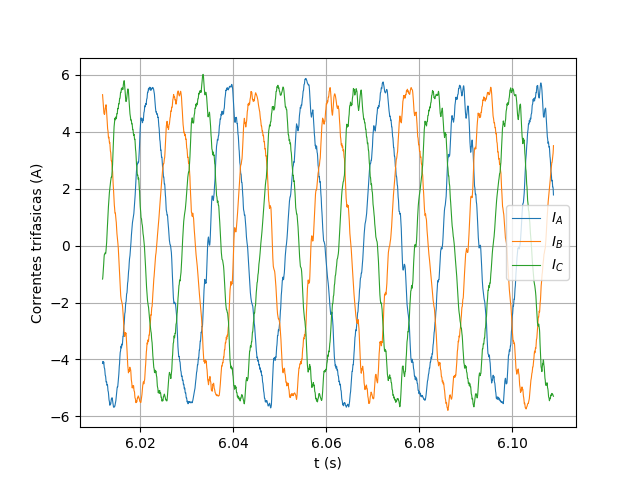
\includegraphics[width=\textwidth]{figuras/sim_figures/inversor_e_boost/corrente_ia_ib_ic.png}
  		\caption{}
 	\end{subfigure}
  	\begin{subfigure}[b]{0.49\textwidth}
  		\centering
  		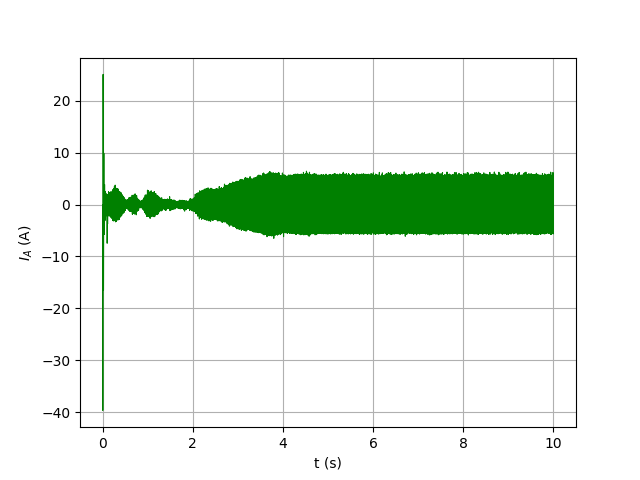
\includegraphics[width=\textwidth]{figuras/sim_figures/inversor_e_boost/injecao_corrente.png}
  		\caption{}
  	\end{subfigure}
     \caption{Análise da corrente de saída após o filtro LCL. Os resultados foram obtidos após a inserção de corrente pelo conversor \textit{boost} no barramento CC: (a) Corrente de saída na fase A. (b) Espectro em frequência da corrente na fase A. (c) Correntes de saída para as fases A, B e C. (d) Aumento da injeção de corrente na rede conforme se injetava potência no inversor.}
     \label{fig:sim-corrente-saida-inversor}
\end{figure}

Na Fig. \ref{fig:sim-tensao-corrente-boost} pode-se verificar os valores de tensão e de corrente na entrada do conversor \textit{Boost}.
É possível ver que a tensão na entrada do conversor é aproximadamente 250 V, e a corrente de entrada aproximadamente 10 A, produzindo desta forma uma potência de entrada $P_{entrada}$ = 2500 W.

Utilizando as Figs. \ref{fig:sim-tensao-saida-inversor} e \ref{fig:sim-corrente-saida-inversor} verifica-se que a tensão de pico é aproximadamente 380 V e que a corrente de pico é aproximadamente 5,2 A.
Desta forma, convertendo para RMS, temos que a tensão RMS é 219,91 V e a corrente RMS 3,7 A. A potência de saída trifásica é, portanto, $P_{saída}$ = $ 3 \times 219,9 \times 3,7$ = 2441 W, mostrando, portanto, que a potência foi transferida, com algumas perdas, para a rede elétrica.

\begin{figure}[!hbt]
	\centering
	\begin{subfigure}[b]{0.49\textwidth}
	\centering
		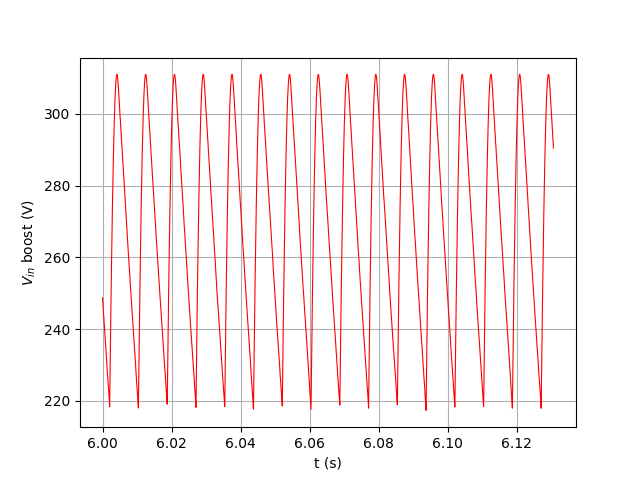
\includegraphics[width=\textwidth]{figuras/sim_figures/inversor_e_boost/tensao_entrada_boost_2.png}
		\caption{}
	\end{subfigure}
	\begin{subfigure}[b]{0.49\textwidth}
	\centering
		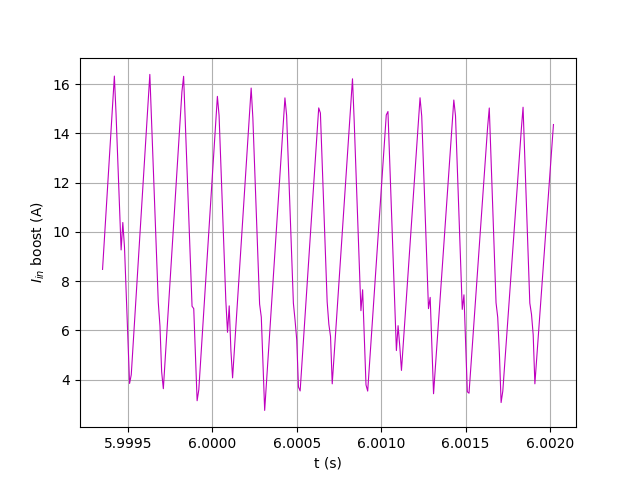
\includegraphics[width=\textwidth]{figuras/sim_figures/inversor_e_boost/corrente_entrada_boost.png}
		\caption{}
	\end{subfigure}
	\begin{subfigure}[b]{0.49\textwidth}
	\centering
		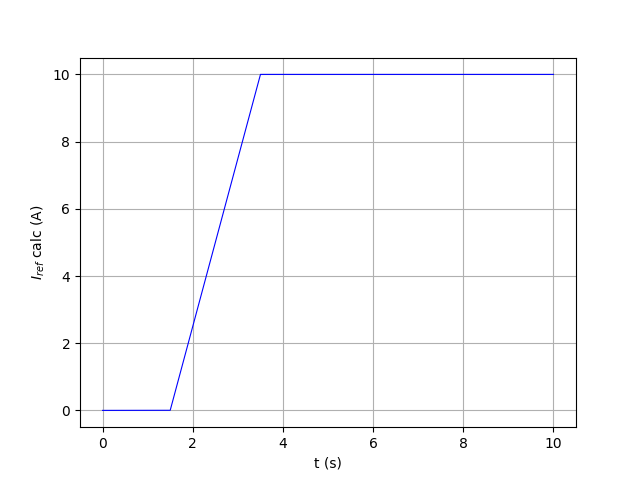
\includegraphics[width=\textwidth]{figuras/sim_figures/inversor_e_boost/corrente_referencia_boost.png}
		\caption{}
	\end{subfigure}
	\caption{Verificação da tensão e corrente de entrada no conversor \textit{Boost} para cálculo da potência de entrada do sistema. (a) Tensão na entrada do conversor \textit{Boost}. (b) Corrente medida na entrada do conversor \textit{Boost}. (c) Referência de corrente para o conversor \textit{boost} mostrando a variação da inserção de corrente no tempo.}
    \label{fig:sim-tensao-corrente-boost}
\end{figure}

\subsection{Comportamento do inversor com a inserção de potência variável no barramento CC}

Nesta etapa de simulação, houve a inserção de corrente variável no barramento CC do 
inversor trifásico através da variação constante da corrente de referência para o conversor 
\textit{boost}, como pode ser verificado no circuito mostrado na Fig. \ref{fig:sim-controle-corrente-esq}.

Neste esquema, a fonte de corrente tratava-se de um onda triangular que injetava potência 
na rede elétrica à uma frequência de 0,125 Hz. A injeção de potência começou a ser realizada 
a partir dos 4 segundos de simulação, como pode ser verificado na Fig. 
\ref{fig:sim-controle-corrente}. A partir disto, pode-se ver que a tensão no barramento de 
corrente contínua permanecia próximo ao valor de referência de 680 V, controlando corretamente
a injeção de potência para a rede elétrica conforme ocorria a variação de corrente na entrada.

A presente simulação atesta o funcionamento do inversor trifásico para aplicações que envolvam 
variações de potência na entrada do barramento, algo comum em aplicações envolvendo geradores 
éolicos e painéis fotovoltaicos.

\begin{figure}[!hbt]
	\begin{center}
    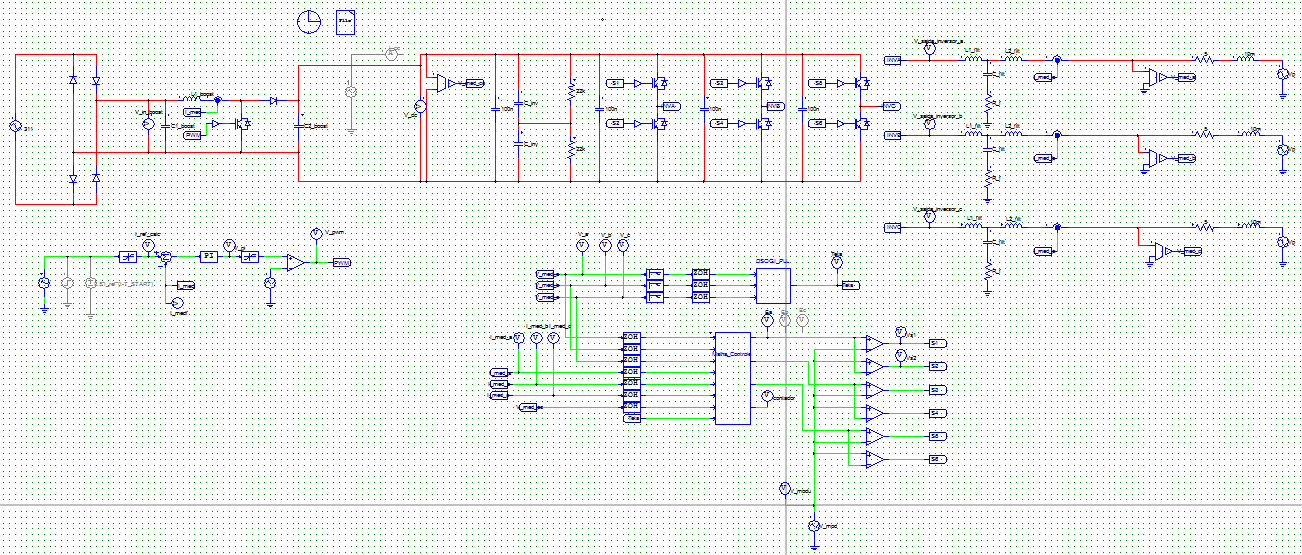
\includegraphics[width=\textwidth]{figuras/sim_figures/inversor_e_boost_variavel/esquematico.PNG}
    \caption{Circuito do inversor trifásico com seu barramento recebendo a injeção de potência variável}
    \label{fig:sim-controle-corrente-esq}
    \end{center}
\end{figure}

\begin{figure}[!hbt]
	\centering
	\begin{subfigure}[b]{0.49\textwidth}
	\centering
		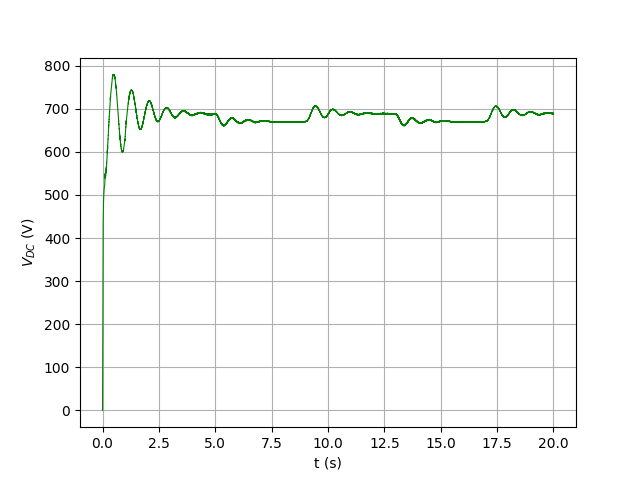
\includegraphics[width=\textwidth]{figuras/sim_figures/inversor_e_boost_variavel/tensao_barramento.png}
		\caption{}
	\end{subfigure}
	\begin{subfigure}[b]{0.49\textwidth}
	\centering
		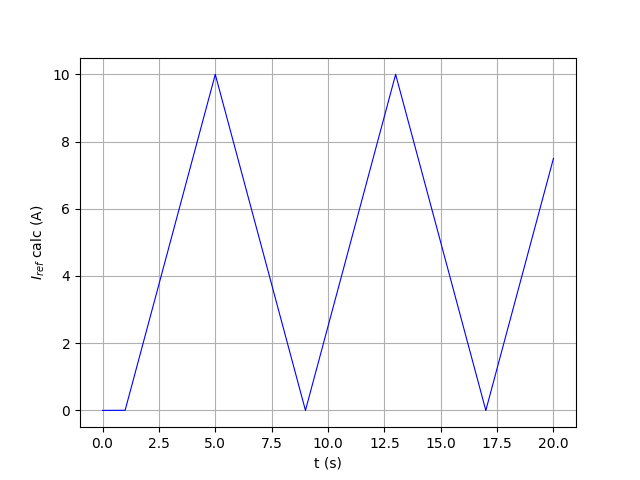
\includegraphics[width=\textwidth]{figuras/sim_figures/inversor_e_boost_variavel/corrente_referencia.png}
		\caption{}
	\end{subfigure}
	\begin{subfigure}[b]{0.49\textwidth}
	\centering
		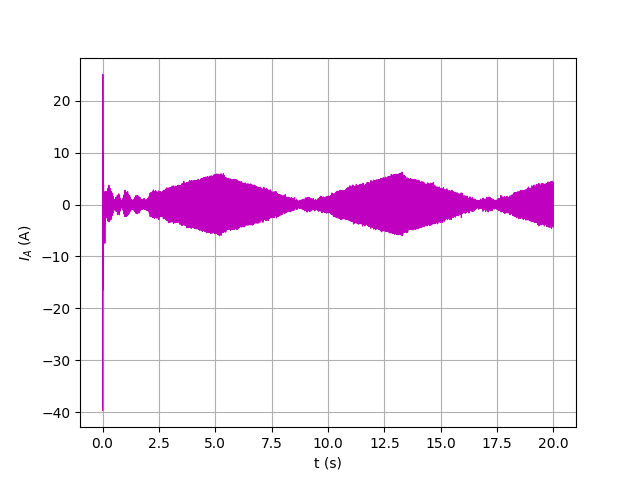
\includegraphics[width=\textwidth]{figuras/sim_figures/inversor_e_boost_variavel/injecao_corrente.png}
		\caption{}
	\end{subfigure}
	\caption{Resultados de simulação para a injeção de uma corrente variável na entrada do barramento CC de 10 A a partir de 1 segundo de simulação: (a) Tensão no barramento CC. (b) Referência de corrente para o conversor \textit{boost}. (c) Injeção de corrente na rede elétrica.}
    \label{fig:sim-controle-corrente}
\end{figure}

\section{Resultados Experimentais}

A Fig. \ref{fig:res-bancada-inversor} apresenta a montagem experimental realizada para validação da bancada.
Esta montagem foi feita utilizando o inversor desacoplado da rede elétrica, de forma que fosse possível validar
os algoritmos de sincronização e de controle. Os testes com o inversor trifásico acoplado à rede elétrica como STATCOM e
utilizando o conversor \textit{boost} ainda estão sendo realizados e não serão abordados neste trabalho.

\begin{figure}[!hbt]
	\begin{center}
    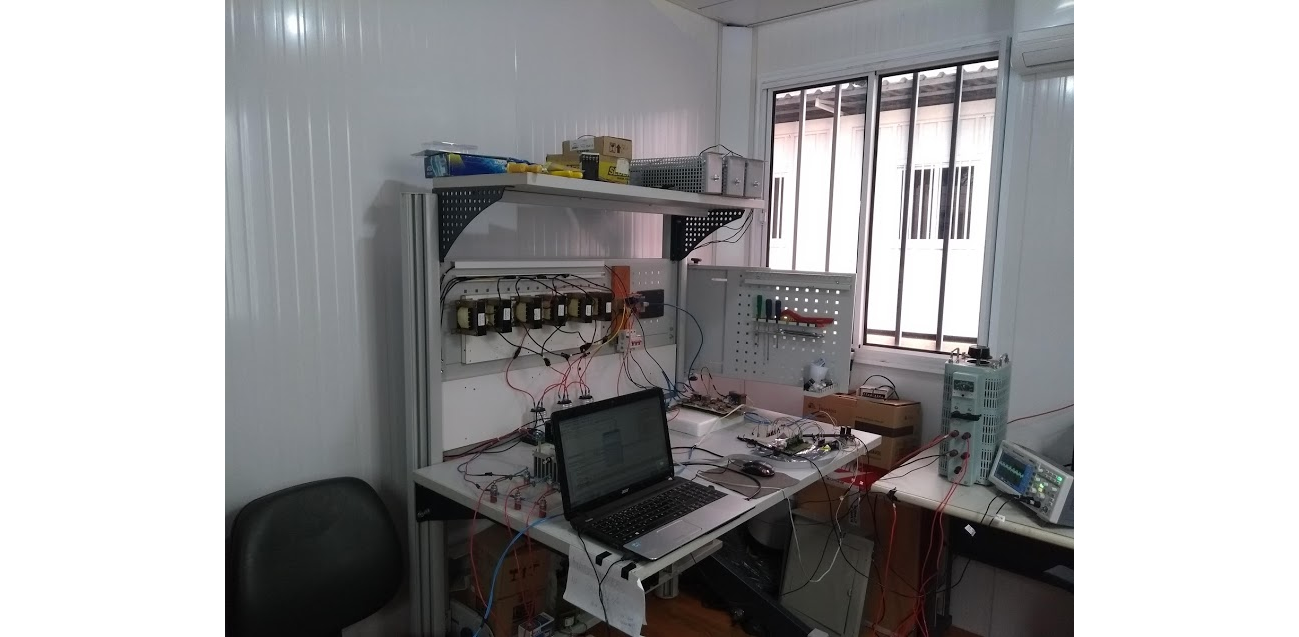
\includegraphics[width=\textwidth]{figuras/resultados-montagem-laboratorial.png}
    \caption{Bancada do inversor trifásico com seus componentes}
    \label{fig:res-bancada-inversor}
    \end{center}
\end{figure}

\subsection{Obtenção e calibração dos sinais de tensão da rede}

A Fig. \ref{fig:res-tensao-va-vb-bc} mostra as tensões da rede elétrica após a etapa de condicionamento de sinais.
Para que as tensões e correntes pudessem ser quantizadas corretamente pelo microcontrolador, 
uma etapa de ajustes finos da placa de condicionamento de sinais foi necessária para que os sinais estivessem dentro da faixa de amostragem do conversor A/D.
Mais especificamente, foi realizado um ajuste através de um \textit{trimpot} que regulava o nível DC dos sinais na entrada do DSP.
Além disso, foi necessário se atentar para a correta sequência de fase da rede elétrica.

\begin{figure}[!hbt]
	\centering
	\begin{subfigure}[b]{0.49\textwidth}
		\centering
		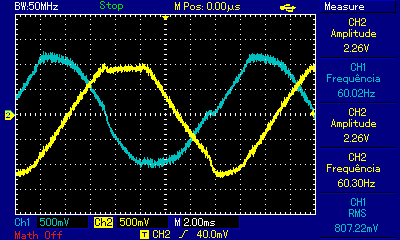
\includegraphics[width=\textwidth]{figuras/resultados_tensao_va_vb.png}
		\caption{}
	\end{subfigure}
	\begin{subfigure}[b]{0.49\textwidth}
		\centering
		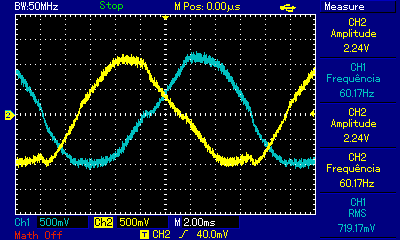
\includegraphics[width=\textwidth]{figuras/resultados_tensao_va_vc.png}
		\caption{}
	\end{subfigure}
	\caption{Verificação dos sinais respectivos às tensões da rede elétrica após a placa de condicionamento de sinais: (a) Tensões $V_A$ (canal 1) e $V_B$ (canal 2). (b) Tensões $V_A$ (canal 1) e $V_C$ (canal 2).}
    \label{fig:res-tensao-va-vb-bc}
\end{figure}

\subsection{Sincronização com a rede elétrica}

A Fig. \ref{fig:res-sincronizacao} mostra a correta sincronização do algoritmo do DSOGI-PLL. 
A GPIO10 do DSP foi configurado como saída digital e no semiciclo positivo da senoide da rede elétrica era acionado (3,3 V) e no semiciclo negativo desativado (0 V).
O canal A do osciloscópio estava conectado ao sensor de tensão da fase $V_A$ da rede elétrica e o canal B estava conectado ao GPIO 10 do DSP.
O ângulo de fase da rede elétrica foi utilizado para o correto acionamento do GPIO, atestando assim o funcionamento do algoritmo em C do DSOGI-PLL no DSP.

\begin{figure}[!hbt]
	\begin{center}
    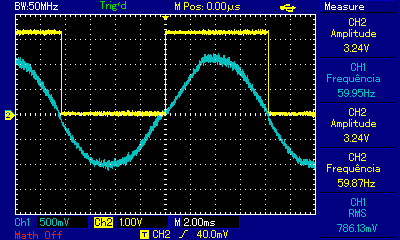
\includegraphics[width=0.4\textwidth]{figuras/resultados_sincronizacao.png}
	\caption{Resultado de sincronização do sistema com a rede elétrica.}
    \label{fig:res-sincronizacao}
    \end{center}
\end{figure}

\subsection{Verificação do SPWM}

Para realização do chaveamento dos IGBTs do inversor, o DSP TMS320F28335 dispõe
de um módulos conhecido como \textit{enhanced Pulse Width Modulation} - ePWM, a qual dispõem de diversas configurações aplicadas à sistemas de potência.
Utilizando o módulo \textit{ePWM}, a frequência de chaveamento foi configurada para 5 kHz e o tempo morto entre os acionamentos dos IGBTs para 10 $\mu s$.
A Fig. \ref{fig:res-pwm} mostra os resultados obtidos. Pode-se verificar que as especificações requeridas foram atendidas.

\begin{figure}[!hbt]
	\centering
	\begin{subfigure}[b]{0.49\textwidth}
		\centering
		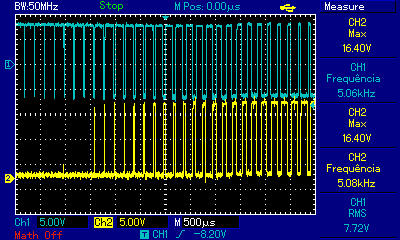
\includegraphics[width=\textwidth]{figuras/resultados_pwm1_1.png}
		\caption{}
	\end{subfigure}
	\begin{subfigure}[b]{0.49\textwidth}
		\centering
		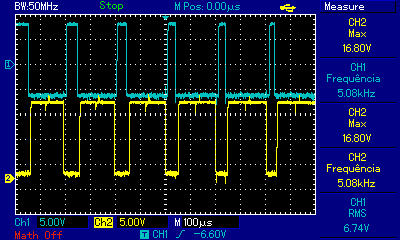
\includegraphics[width=\textwidth]{figuras/resultados_pwm2_1.png}
		\caption{}
	\end{subfigure}
	\begin{subfigure}[b]{0.49\textwidth}
		\centering
		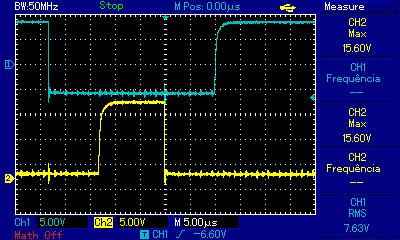
\includegraphics[width=\textwidth]{figuras/resultados_tempo_morto1.png}
		\caption{}
	\end{subfigure}
	\begin{subfigure}[b]{0.49\textwidth}
		\centering
		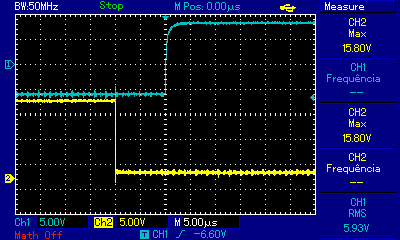
\includegraphics[width=\textwidth]{figuras/resultados_tempo_morto2.png}
		\caption{}
	\end{subfigure}
	\caption{Sinal de PWM amplificado após a placa de conversão dos sinais de 3,3V para 15V: (a) Forma de onda do PWM trifásico. (b) Aproximação na forma de onda. (c) Aproximação mais detalhada para demonstrar o tempo morto configurado. (d) Verificação do tempo morto de 10 $\mu s$.}
    \label{fig:res-pwm}
\end{figure}

\subsection{Validação da malha de controle de corrente}

Para validação da malha de controle de corrente, foi criado um teste em C em que a corrente de referência em eixo direto $I_{d,ref}$ 
foi variada a cada 5 segundos, de forma que esta era inicializada em 0,3 A, após 5 segundos, passava para 0,6 A e assim sucessivamente,
até atingir 1,5 A, e depois voltava para 0,3 A, em um esquema de escada.

Assim, verificou-se a corrente enviada para os resistores de 100 $\Omega$ com o alicate amperímetro e a Tab. \ref{tab:res-controle-corrente} foi montada.
Pode-se verificar que a corrente medida no alicate amperímetro tem uma amplitude próxima da corrente desejada, demonstrando assim que a malha de controle de corrente
estava funcionando. Os erros entre os valores medidos e esperados são devidos, principalmente, as perdas nos componentes elétricos.

\begin{table}[h]
	\centering
	\caption{Resultados para atestar o funcionamento da malha de controle de corrente. Os passos foram dados a cada 5 segundos.}
	\label{tab:res-controle-corrente}
	
	\begin{tabular}{m{5cm}m{5cm}m{5cm}}
		\toprule
		\multicolumn{3}{c}{\textbf{Tensão no barramento CC:} 308 V} \\
		\textbf{Corrente Esperada (A)} & \textbf{Corrente Medida (A)} & \textbf{Tensão sintetizada pelo inversor (V)}\\
		\midrule
		\multicolumn{1}{c}{0,3} & \multicolumn{1}{c}{0,225} & \multicolumn{1}{c}{40} \\
		\multicolumn{1}{c}{0,6} & \multicolumn{1}{c}{0,460} & \multicolumn{1}{c}{82} \\
		\multicolumn{1}{c}{0,9} & \multicolumn{1}{c}{0,693} & \multicolumn{1}{c}{124} \\
		\multicolumn{1}{c}{1,2} & \multicolumn{1}{c}{0,930} & \multicolumn{1}{c}{167} \\
		\multicolumn{1}{c}{1,5} & \multicolumn{1}{c}{1,173} & \multicolumn{1}{c}{209} \\
		\bottomrule
	\end{tabular}
\end{table}

A Fig. \ref{fig:res-controle-corrente} mostra a variação na amplitude da corrente medida pelo trandutor e placa de condionamento de sinais a cada 5 segundos. 
No canal 1 está o sinal de corrente lido após a placa de condicionamento de sinais e no canal 2 o GPIO10, que é ativado nos semiciclos positivos da PLL, mostrando que a corrente está em fase com a tensão da rede.
e a Fig. \ref{fig:res-escada-corrente} mostra a variação da amplitude de corrente no tempo demonstrando assim o correto controle da malha.

\begin{figure}[!hbt]
	\centering
	\begin{subfigure}[b]{0.49\textwidth}
		\centering
		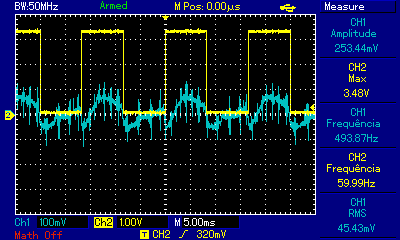
\includegraphics[width=\textwidth]{figuras/resultados_controle_corrente_0_3.png}
		\caption{}
	\end{subfigure}
	\begin{subfigure}[b]{0.49\textwidth}
		\centering
		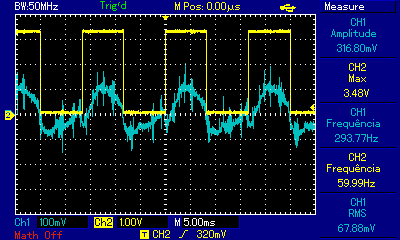
\includegraphics[width=\textwidth]{figuras/resultados_controle_corrente_0_6.png}
		\caption{}
	\end{subfigure}
	\begin{subfigure}[b]{0.49\textwidth}
		\centering
		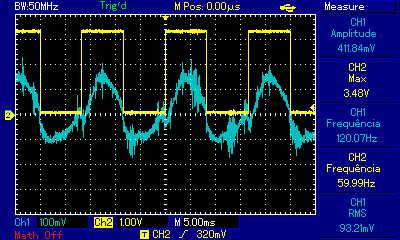
\includegraphics[width=\textwidth]{figuras/resultados_controle_corrente_0_9.png}
		\caption{}
	\end{subfigure}
	\begin{subfigure}[b]{0.49\textwidth}
		\centering
		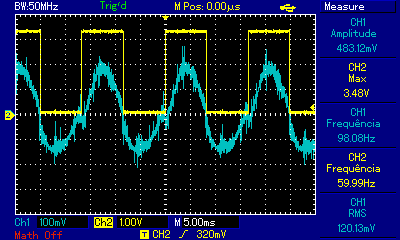
\includegraphics[width=\textwidth]{figuras/resultados_controle_corrente_1_2.png}
		\caption{}
	\end{subfigure}
	\begin{subfigure}[b]{0.49\textwidth}
		\centering
		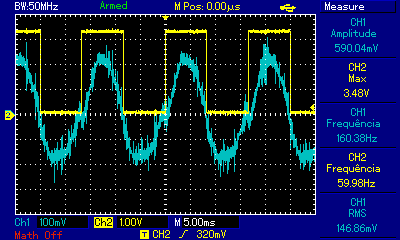
\includegraphics[width=\textwidth]{figuras/resultados_controle_corrente_1_5.png}
		\caption{}
	\end{subfigure}
	\caption{Verificação do aumento da amplitude no sinal de corrente: (a) Resultado para $I_{d,ref}$ = 0,3 A. (b) Resultado para $I_{d,ref}$ = 0,6 A. (c) Resultado para $I_{d,ref}$ = 0,9 A. (d) Resultado para $I_{d,ref}$ = 1,2 A. (e) Resultado para $I_{d,ref}$ = 1,5 A.}
    \label{fig:res-controle-corrente}
\end{figure}

\begin{figure}[!hbt]
	\begin{center}
    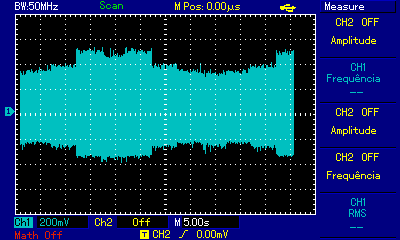
\includegraphics[width=0.4\textwidth]{figuras/resultados_escada_corrente.png}
	\caption{Escada de corrente no tempo mostrando a variação de amplitude a cada 5 segundos}
    \label{fig:res-escada-corrente}
    \end{center}
\end{figure}
